\documentclass[10pt,twocolumn,letterpaper]{article}

\usepackage{cvpr}
\usepackage{times}
\usepackage{epsfig}
\usepackage{graphicx}
\usepackage{amsmath}
\usepackage{amssymb}
\usepackage{graphicx}
\usepackage[utf8]{inputenc}
\usepackage[T1]{fontenc}
\usepackage{lmodern} % load a font with all the characters
\usepackage[justification=centering]{caption}
\usepackage{float}
\usepackage{enumitem}
\usepackage{caption}
\usepackage{lipsum}
\usepackage{titlesec}
\captionsetup[figure]{name=Figura}

% Include other packages here, before hyperref.

% If you comment hyperref and then uncomment it, you should delete
% egpaper.aux before re-running latex.  (Or just hit 'q' on the first latex
% run, let it finish, and you should be clear).
\usepackage[breaklinks=true,bookmarks=false]{hyperref}

\cvprfinalcopy % *** Uncomment this line for the final submission

\def\cvprPaperID{****} % *** Enter the CVPR Paper ID here
\def\httilde{\mbox{\tt\raisebox{-.5ex}{\symbol{126}}}}

% Pages are numbered in submission mode, and unnumbered in camera-ready
%\ifcvprfinal\pagestyle{empty}\fi
\setcounter{page}{1}

\begin{document}

%%%%%%%%% TITLE
\title{Laboratorio 5: Segmentación en base de datos BSDS500}

\author{Juliana de la Vega Fernández\\
código 201312387\\
Departamento de Ingeniería Biomédica\\
Universidad de los Andes\\
{\tt\small j.de10@uniandes.edu.co}}
% For a paper whose authors are all at the same institution,
% omit the following lines up until the closing ``}''.
% Additional authors and addresses can be added with ``\and'',
% just like the second author.
% To save space, use either the email address or home page, not both


\maketitle
%\thispagestyle{empty}

%%%%%%%%% ABSTRACT
\begin{abstract}
   En este artículo se presentan los resultados de la segmentación realizada por la función segment\_by\_clustering.m. Los resultados de dicha función se obtienen al aplicarla en la base de datos BSDS500 de la Universidad de California Berkeley. Las segmentaciones se comparan con la verdad terreno de la base de datos y se obtienen las curvas de precisión y cobertura. El algoritmo evalúa la según el espacio de colores empleado, el algoritmo de segmentación, y el número de clústeres. Los resultados demuestran la superioridad de la segmentación al emplear un espacio de color perceptualmente uniforme, y además exhibe una medida F mayor para la segmentación de tipo watersheds. 
\end{abstract}

%%%%%%%%% BODY TEXT
\section{\textbf{I. Introducción}}

La segmentación de imágenes corresponde a la tarea de visión artificial que se dedica a encontrar grupos de píxeles que conforman un mismo grupo [1]. En la actualidad existen muchos algoritmos que ofrecen una aproximación al problema. En este artículo se evalúan tres diferentes algoritmos, Watersheds, K-means y Segmentación Jerárquica en la base de imágenes BSDS500 de la Universidad de California Berkeley. La base de datos BSDS500 es una extensión de la base BSDS300 en la cual se emplean las 300 imágenes originales para entrenamiento y validación, y 200 imágenes nuevas para prueba [2]. Cada una de estas imágenes fue segmentada por cinco personas, las cuales se emplean como verdad terreno. Las imágenes fueron segmentadas con los algoritmos previamente mencionados empleando diferentes espacios de color.  Una vez segmentadas, se emplea otro algoritmo para evaluar la segmentación producida en comparación con la realizada por los humanos. A continuación se describe los algoritmos de segmentación, y los espacios de color empleados en este laboratorio.

%-------------------------------------------------------------------------
\subsection{\textit{A. Algoritmos de segmentación}}

\subsubsection*{ Watersheds}
La técnica de Watersheds opera sobre imágenes en escala de grises. La imagen se segmenta en diferentes catchment basins las cuales son regiones de una imagen donde la lluvia fluiría hacia un mismo lago [1]. Vincent y Soille en 1991 desarrollaron un algoritmo para computar los catchment basins. En su algoritmo, se realizaba una inundación de la imagen desde todos los mínimos locales, y se delimitaban las regiones donde dos o más lagos presentaban uniones. Sin embargo, los watersheds presentan un problema, debido a que se emplean mínimos locales se obtiene una sobre segmentación de la imagen. Es por esto que se implementa watersheds jerárquico, donde se intenta disminuir la sobre segmentación al unir regiones que están muy cercanas entre sí [1].
En este caso, el algoritmo empleado emplea la función de Matlab \textit{imextendedmin} para seleccionar un nivel en la jerarquía de unión de los mínimos de la imagen, y a partir de estos se realiza el watershed. De esta manera se logra automatizar el proceso de segmentación con watersheds, disminuyendo la sobre segmentación mencionada anteriormente.

\subsubsection*{ K-means}

La segmentación mediante k-means emplea un modelo paramétrico de la función de probabilidad en la que se asume que esta tiene distribuciones esféricas [1]. El algoritmo de k-means requiere que se defina el número k de clúster que debe encontrar en la imagen. Posteriormente, mediante la iteración se determina el centroide de cada clúster empleando las muestras más cercanas a los centros [1].
Debido a que k-means corresponde a clasificación no supervisada, en el algoritmo el primer paso es asignas de manera aleatoria la ubicación de los k centroides [1]. Luego, mediante un diagrama de Voronoi se asignan los elementos que corresponden a cada clúster. Con los elementos de cada clúster se realiza la computación del nuevo centroide. Estos últimos dos pasos se repiten iterativamente hasta que se logre estabilidad en la asignación del centroide. Este algoritmo se conoce como \textit{Lloyd’s Algorithm} [1].

\subsubsection*{ Segmentación Jerárquica}
La segmentación jerárquica se fundamenta en la definición de distancias entre grupos se basa en la similaridad entre los elementos. Con estas distancias se crea una jerarquía de las particiones; dicha jerarquía puede ser representada por un dendrograma. En este artículo se emplea distancias que miden la similaridad entre centroides, es decir, distancia euclidea. Aunque existen otros modelos de vinculación, este fue el empleado  en el código de segmentación [3].
El algoritmo inicialmente define cada pixel de la imagen como correspondiente a un clúster diferente, y procede a unir los clústeres más cercanos entre sí. Esta unión se repite iterativamente hasta que solo exista un clúster en la imagen. Así es como se obtiene una jerarquía dentro de la imagen, donde las primeras uniones representan distancias muy cortas, y por ende tendrán un índice menor; y las últimas uniones representan largas distancias, con un índice superior. Para la selección de la jerarquía se elige un máximo número de clústeres que puedan existir en la imagen, y se realiza la segmentación de la imagen basándose en los bordes que han sobrevivido hasta este punto. En el dendrograma  resulta más clara la representación del máximo número de clústeres, como se observa en la figura 1.
 \begin{figure}[H]
\begin{center}
   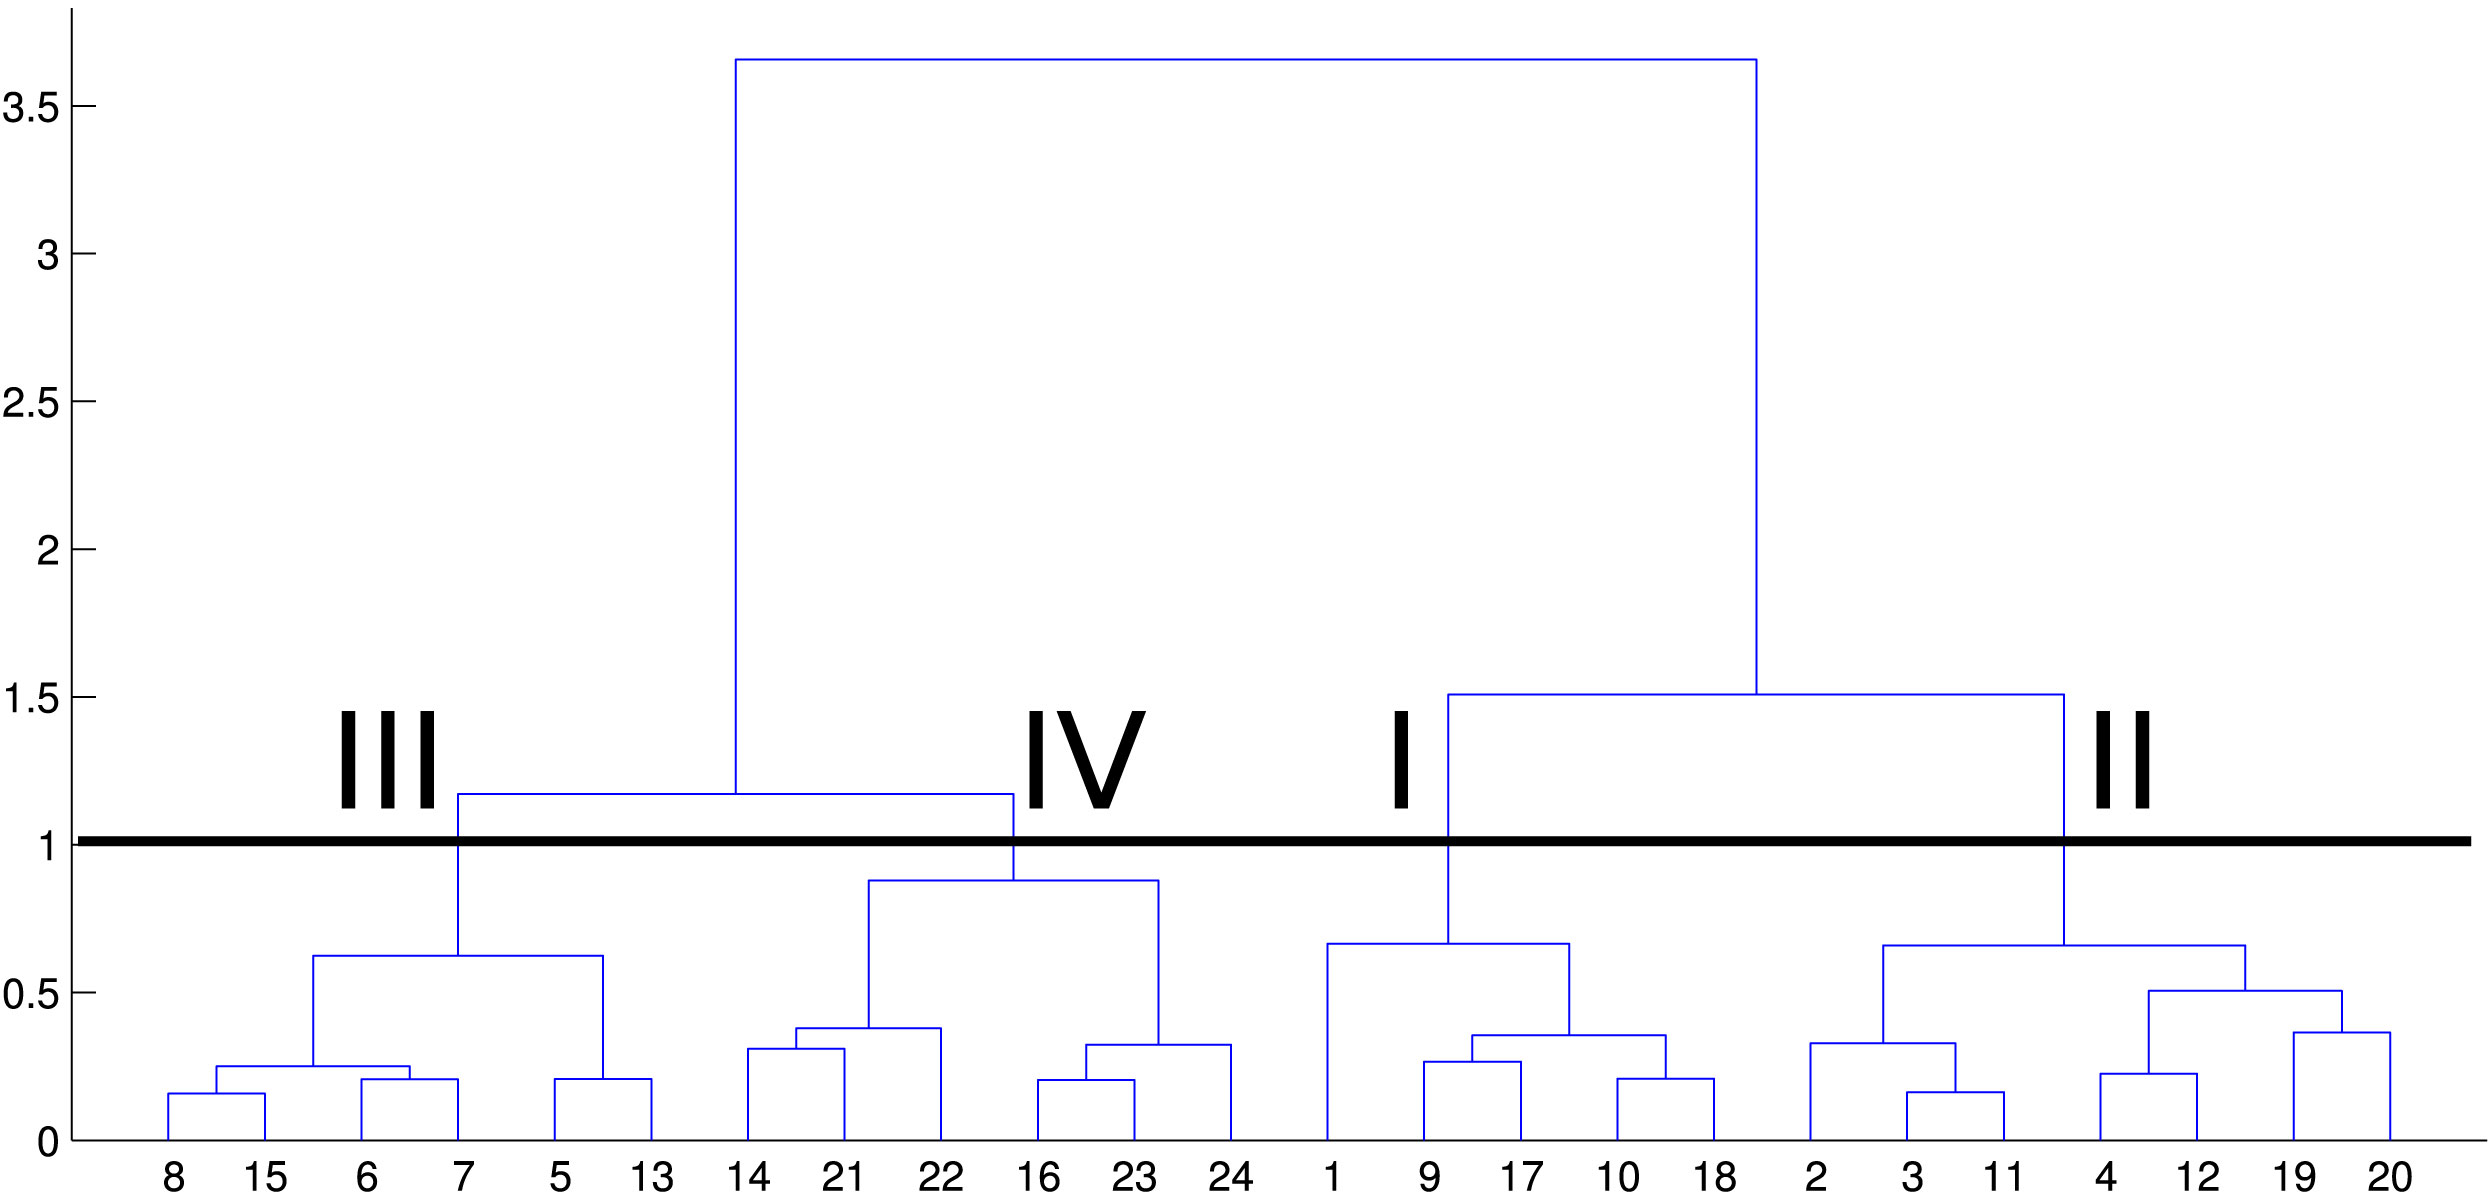
\includegraphics[scale = 0.1]{klobucar}
\end{center}
   \caption{Ejemplo de dendrograma, tomado de:(Klobucar, Subastic, 2012) }
\end{figure}

\subsection{\textit{B. Espacios de Color}}

Cada uno de los métodos anteriormente descritos presenta variaciones en sus respuestas dependiendo del espacio de color utilizado. Aunque hace algunos años existía preferencia por el espacio de color RGB, hoy día existen espacios que son perceptualmente uniforme, ofreciendo una mayor correlación entre las distancias que existen entre los colores. También se emplea el espacio de color HSV, que aunque no corresponde a la categoría de perceptualmente uniforme, ofrece una relación no lineal entre colores. A continuación se encuentra una descripción más detallada [4].

\subsubsection*{ HSV}
Siglas de Hue, Saturation, Value, en español corresponden a Tono, Saturación y Valor el cual es un espacio de color no lineal. Este espacio de color se representa mediante un cono. El tono corresponde al ángulo en la sección cónica, en 0º se encuentra el color Rojo, en 120º se encuentra el color verde, en 240º el color azul, y en grados intermedios están los demás colores.  La saturación corresponde a la distancia entre al eje del cono, y hace referencia a la pureza del color. El valor es el eje del cono, la punta del cono corresponde al negro, y la base del cono corresponde al blanco [4].
 \begin{figure}[H]
\begin{center}
   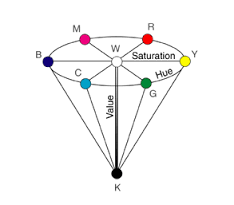
\includegraphics[scale = 0.65]{images}
\end{center}
   \caption{Representación del espacio de color HSV, tomado de:\url{https://www.e-education.psu.edu/geog486/node/1861} }
\end{figure}

\subsubsection*{ La*b*}
Corresponde a un espacio de color perceptualmente uniforme, donde las distancias entre colores es euclidea. L a* b* se representa mediante una esfera, cuyo eje corresponde a la luminancia, y los ejes a* y b*, ortogonales entre sí, corresponden a la crominancia. El canal a* varía de rojo hasta verde puros, y el canal b* varía de azul a amarillo puro.  La transformación de RGB a La*b* se puede realizar mediante recursos del álgebra lineal [4].

 \begin{figure}[H]
\begin{center}
   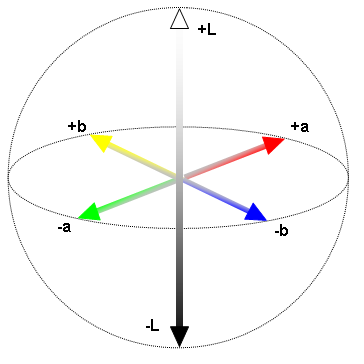
\includegraphics[scale = 0.45]{CIE_Lab.png}}
\end{center}
   \caption{Representación del espacio de color La*b*, tomado de:\url{http://www.codeproject.com/Articles/243610/The-Known-Colors-Palette-Tool-Revised} }
\end{figure}

\section{\textbf{II. Metodología}}
Los anteriores algoritmos se emplearon de la siguiente manera:
•	Watersheds en espacio de color La*b* , se realizó una primera implementación con k’s de {2 6 10 14 18 22 26 30 34 38 42 46 50 54 58} sobre la base de datos de entrenamiento (train) de BSDS500.
•	K-means en el espacio de color HSV con asignación de k centroides que variaban de {2 6 10 14 18 22 26 30 34 38}. Se implementó sobre la base de datos de entrenamiento (train) de BSDS500.
•	Segmentación Jerárquica en el espacio de color La*b*, con k máximos clústeres, que varían entre {2 6 10 14 18 22 26 30 34 38}. Se implementó sobre la base de datos de entrenamiento (train) de BSDS500.

Posteriormente se seleccionaron los dos métodos con mejores curvas de precisión cobertura para realizar las pruebas sobre la base de datos de test de BSDS500. Estos fueron watersheds y k-means. Para ambos se incrementó el número de k’s empleados hasta, y los pasos entre cada k se redujeron a 2, realizando pasos de 2 a 100.

\subsection{ \textit{A. Desarrollo del algoritmo \textit{segment\_by\_clustering.m}}}
Se implementó el algoritmo \textit{segment\_by\_clustering.m }en Matlab, el cual es una función que recibe como parámetros la imagen de entrada, el espacio de color a evaluar, el método de segmentación, y el número de clústeres a utilizar. La imagen de entrada que recibe la función se asume que está en el espacio de color RGB. El espacio de color a utilizar puede ser: RGB, La*b*, HSV, y los mismos espacios considerando la distancia, RGB+XY, La*b*+XY, y HSV+XY. 

El método de segmentación que elije el usuario puede corresponder a: k-means, GMM (modelo de distribución de gaussianas), segmentación jerárquica o watersheds.  El algoritmo inicialmente fue verificado empleando cinco imágenes, un ejemplo de estas se puede observar en la figura 4. El resultado se puede observar en las figuras 5 a 8.

\begin{figure}[H]
\begin{center}
   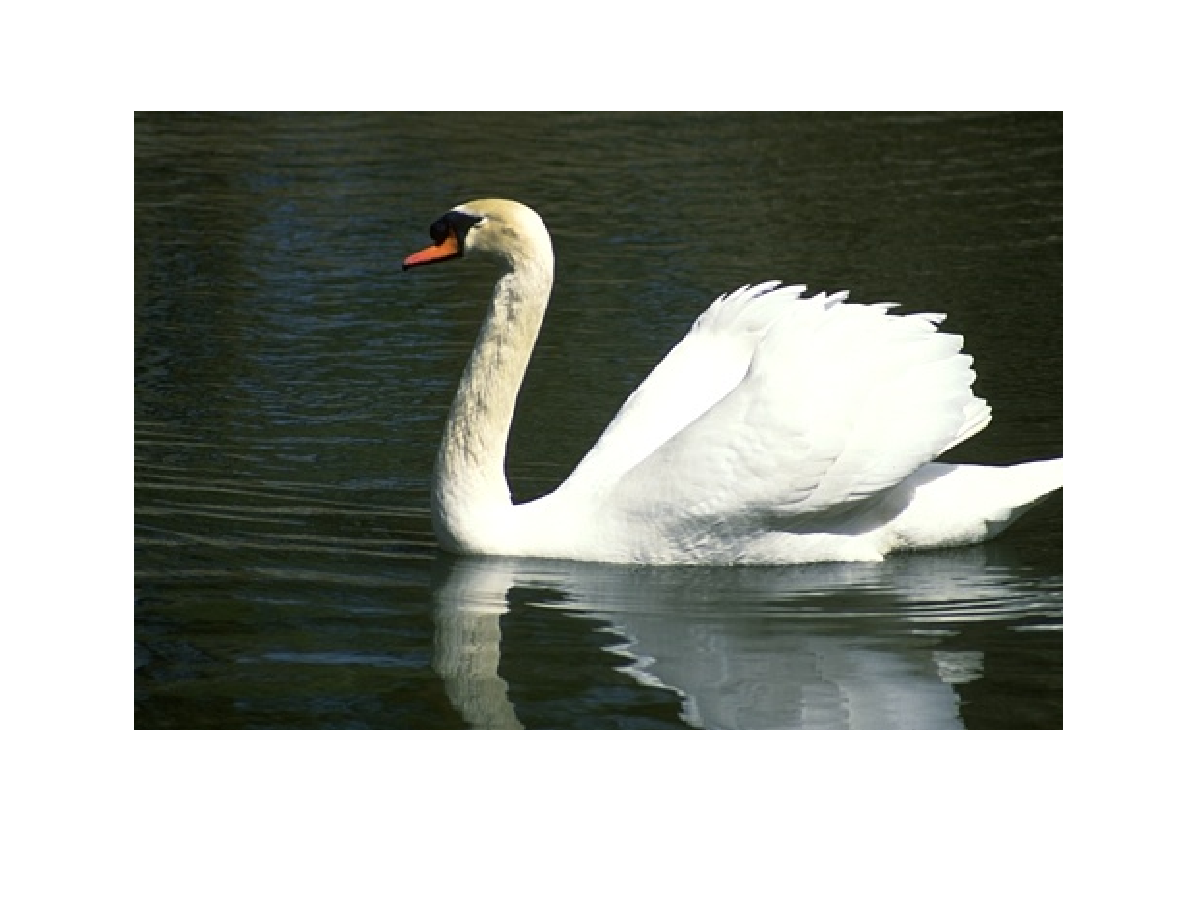
\includegraphics[scale = 0.45]{imagenPrueba}
\end{center}
   \caption{Imagen de prueba original de la base de datos BSDS}
\end{figure}

Se seleccionaron los métodos k-means, hierarchical y watersheds debido a su desempeño en cuanto a la segmentación obtenida con las imágenes, y los espacios de colores se seleccionaron buscando el mejor resultado de la segmentación buscando la relación con las distancias de color. Aunque habría sido de mucha utilidad considerar las distancias en el espacio de la imagen, el tiempo de procesamiento para dichos espacios prolongaba las horas de la prueba. La salida de la función segment_by_clustering.m es la imagen segmentada.

\begin{figure}
\begin{center}
   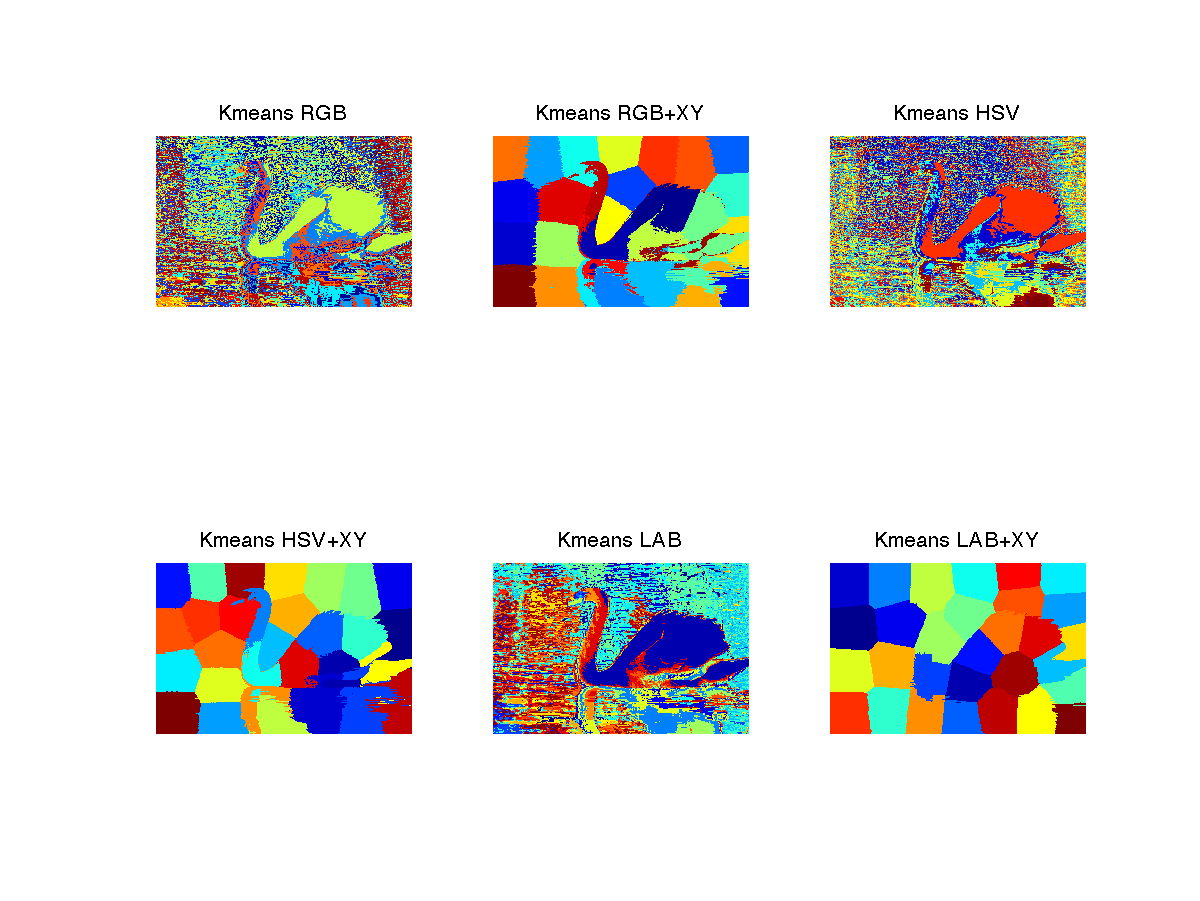
\includegraphics[scale = 0.40]{segmentacionsPruebaKmeans}
\end{center}
   \caption{Imagenes de segmentación mediante algoritmo de Kmeans utilizando espacios de color RGB, RGB+XY, HSV, HSV+XY, LAB, y LAB+XY, empleando 30 clusters}
\end{figure}

\begin{figure}
\begin{center}
   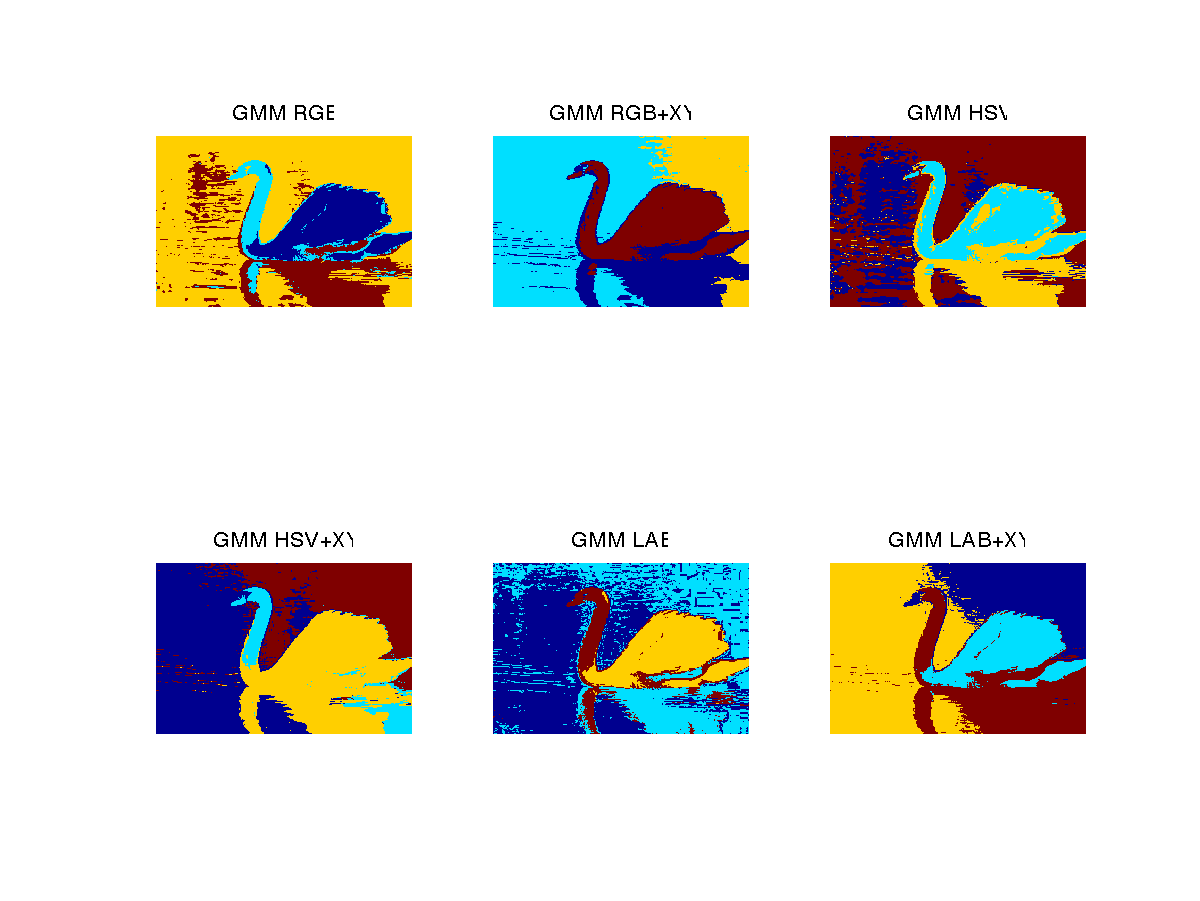
\includegraphics[scale = 0.40]{segmentacionsPruebaGMM}
\end{center}
   \caption{Imagenes de segmentación mediante algoritmo de GMM utilizando espacios de color RGB, RGB+XY, HSV, HSV+XY, LAB, y LAB+XY, empleando 4 clusters}
\end{figure}

\begin{figure}
\begin{center}
   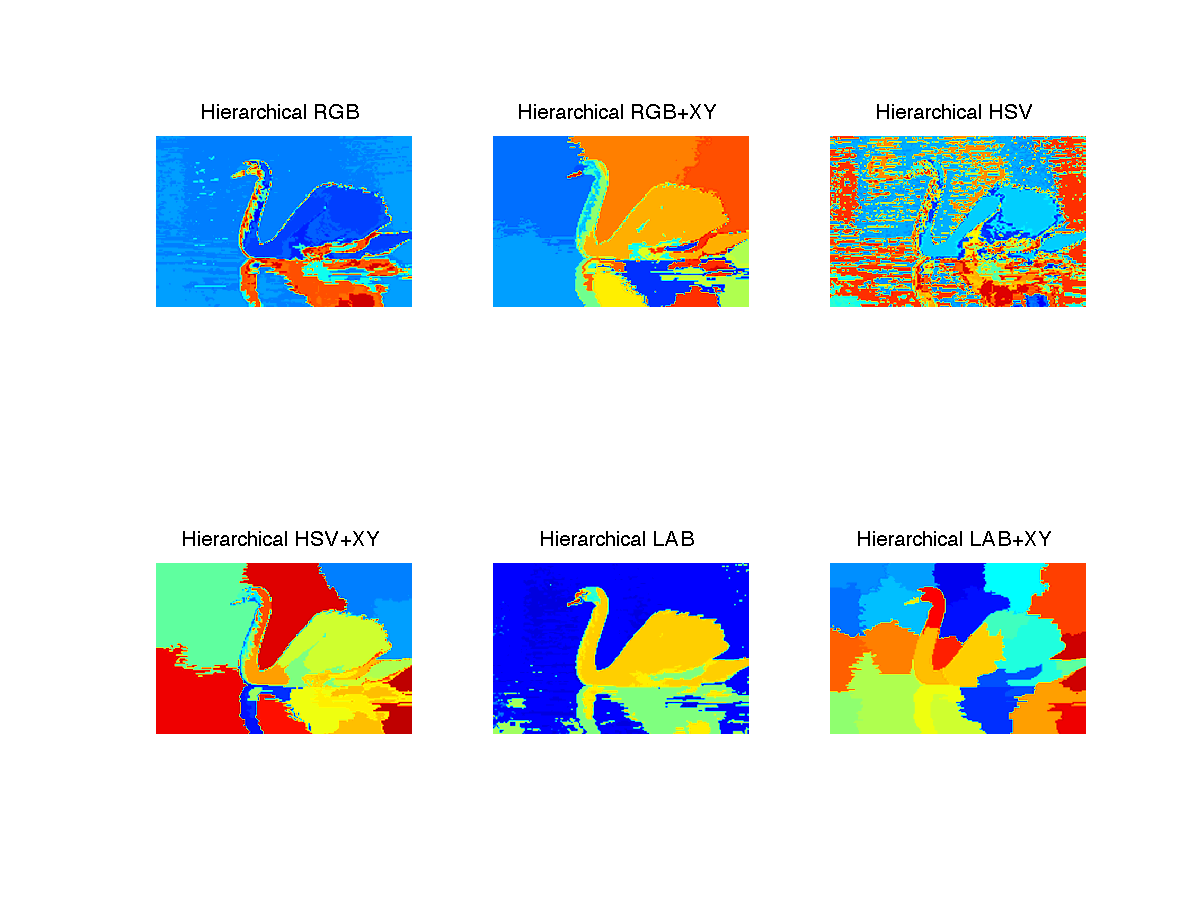
\includegraphics[scale = 0.40]{segmentacionsPruebaHierarchical}
\end{center}
   \caption{Imagenes de segmentación mediante algoritmo de segmentación Jerárquica utilizando espacios de color RGB, RGB+XY, HSV, HSV+XY, LAB, y LAB+XY, empleando 30 clusters}
\end{figure}

\begin{figure}
\begin{center}
   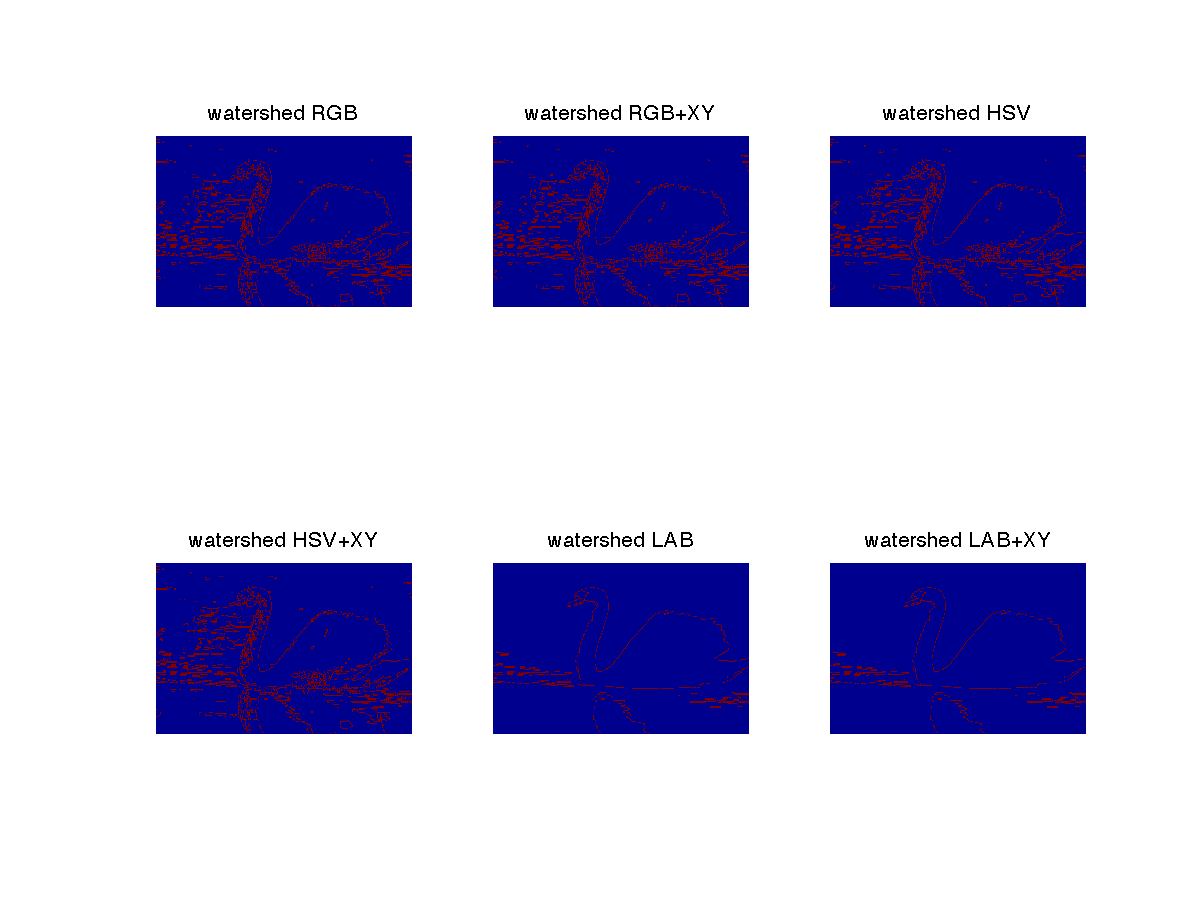
\includegraphics[scale = 0.40]{segmentacionsPruebaWatershed}
\end{center}
   \caption{Imagenes de segmentación mediante algoritmo de Watersheds utilizando espacios de color RGB, RGB+XY, HSV, HSV+XY, LAB, y LAB+XY, empleando 30 clusters}
\end{figure}

\subsection{ \textit{B. Desarrollo del algoritmo \textit{generateSegmentations.m}}}
La prueba sobre la totalidad de las 200 imágenes en la base de datos de entrenamiento y las 200 imágenes de la base de datos de prueba de BSDS500 se realizó mediante el algoritmo generateSegmentations.m, el cual iterativamente seleccionaba las imágenes de la base de datos y las pasaba por la función previamente mencionada segment\_by\_clustering.m, pasando por los números de k previamente descritos para cada base de datos. Por último, el algoritmo guarda todas las segmentaciones de la imagen en una estructura de celdas. 

\subsection{ \textit{C. Evaluación de las segmentaciones realizadas}}
Para la evaluación de las segmentaciones realizadas se empleó el algoritmo proporcionado con la base de datos BSDS500, \textit{test\_benchs.m}. Empleando el numeral 3 del código, se evaluó las segmentaciones obtenidas con la verdad terreno de la base de datos correspondiente. La salida del algoritmo corresponde a tres archivos de texto, eval\_bdry\_thr.txt, eval\_bdry.txt y eval\_cover.txt. El directorio con estos tres archivos se introduce al algoritmo \textit{plot\_eval.m} en el cual se obtienen las gráficas de precisión y cobertura de las segmentaciones en comparación a la verdad terreno. Matemáticamente, la precisión y la cobertura corresponden a:
\begin{center}
	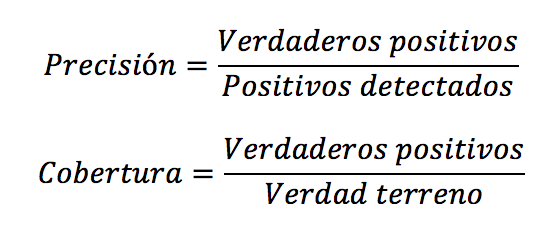
\includegraphics[scale=0.25]{eqn1.png}}
\end{center}
donde los positivos detectados corresponden a verdaderos positivos y falsos positivos, y verdad terreno corresponde a los verdaderos positivos y falsos negativos.  El valor numérico para la comparación de dichas curvas corresponde al valor F, el cual es el punto de máxima precisión y cobertura de la curva. Dicho valor se obtiene de la siguiente manera:
\begin{center}
	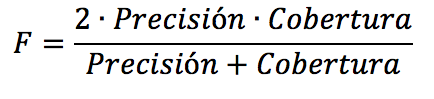
\includegraphics[scale=0.25]{eqn2.png}}
\end{center}

\section{\textbf{ III. Resultados}}
En el entrenamiento de la función de segmentación se obtuvo la siguiente curva de precisión y cobertura:
\begin{figure}[H]
\begin{center}
   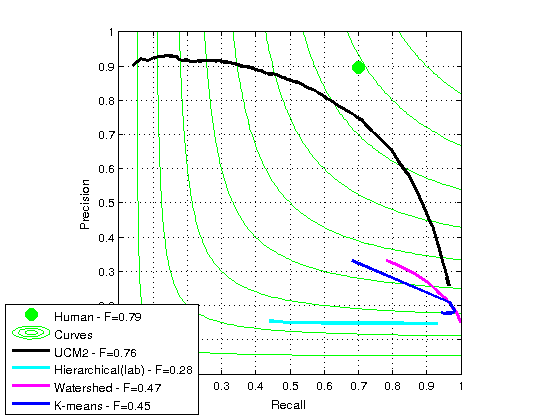
\includegraphics[scale = 0.65]{curves_1}
\end{center}
   \caption{Curva de Precisión vs Cobertura para las segmentaciones de la base de datos de entrenamiento. El máximo F corresponde a watersheds en espacio de color La*b*, con un valor de 0.47}
\end{figure}

En esta curva se observa que la segmentación jerárquica empleada no presenta mayores variaciones en la precisión, sin embargo disminuye la cobertura con el número de k ‘s elegidos. Las curvas para k-means y watersheds están muy cercanas entre sí, sin embargo la segmentación de watersheds aumenta la precisión, superando al menos en 2\% el F máximo que aquel obtenido con k-means. La segmentación empleando UCM2 sigue siendo mucho mejor que aquella de alguno de los otros tres métodos utilizados.

Basado en los resultados anteriores, se procede a segmentar las imágenes de la base de datos de prueba, empleando más iteraciones en la variable de clústeres, k. Esto se realizó únicamente con los algoritmos de k-means y watersheds. El siguiente fue el resultado obtenido:

\begin{figure}[H]
\begin{center}
   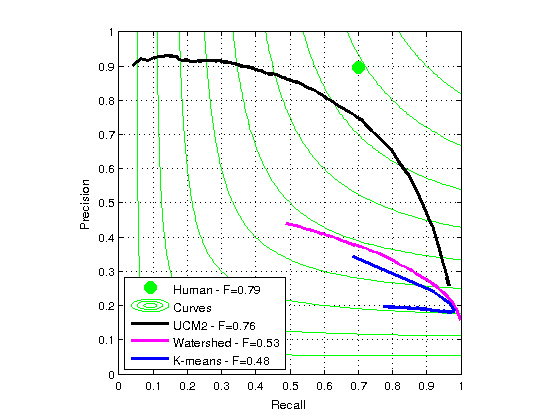
\includegraphics[scale = 0.65]{curve2}
\end{center}
   \caption{Curva de Precisión vs Cobertura para las segmentaciones de la base de datos de prueba. El máximo F corresponde a watersheds en espacio de color La*b*, con un valor de 0.53}
\end{figure}

Los resultados obtenidos con la segmentación sobre la base de datos de prueba, y aumentando el número de clusters evaluado demuestran un F máximo superior a aquel que demuestran las segmentaciones con la base de datos de entrenamiento. En la figura 10 y en la 9 también se observan unas curvas claras verdes, cualquier punto en una de estas curvas continuas tienen una misma medida F. El punto único sobre las gráficas representan la precisión y cobertura de los 5 humanos en la base de datos BSDS500. 

\section{\textbf{IV. Discusión}}
De acuerdo a la teoría, los métodos de segmentación de Jerárquica y Watersheds, al ser mas complejos, deberían tener mejores resultados respecto a los métodos de k-means y GMM. En los resultados se observa que Watersheds si demuestra un mejor resultado respecto a k-means, sin embargo k-means presenta mejores resultados que la segmentación jerárquica. Lo anterior se puede deber a que debido al tiempo de corrido, se redujo el tamaño de la imagen al 40\%, lo cual a su vez reduce la calidad de la misma.

En cuanto a los espacios de color, se esperaba que emplear el espacio de color La*b*, el cual es perceptualmente uniforme, se lograra un resultado en la segmentación con mayor similitud a la verdad terreno. El resultado fue satisfactorio, pues el método que empleaba el espacio de color La*b* demostró superioridad respecto al método en espacio de color HSV, sin embargo, para realizar una comparación adecuada, se debe emplear el mismo método de segmentación empleando los diferentes espacios de color. 

Aunque el resultado esperado sería obtener precisión de 1.00 y cobertura de 1.00, las segmentaciones producidas por los humanos corresponden a una medida F del 0.79, lo cual se traduce a 70\% de cobertura y 90\% de precisión. El método de watersheds es el que demuestra mayor cercanía, con una medida F de 0.53. Sin embargo, es superado por el método UCM con una medida F de 0.76, la cual es solo se aleja en 0.03 de la medida F de las segmentaciones humanas.

Aun así, los métodos K-means y watersheds presentan medidas F muy cercanas entre sí. Sin embargo, para compararlas directamente sería necesario emplear el mismo espacio de color en ambas. Probablemente K-means demuestre un desempeño menor debido a sus limitaciones, como la de converger en mínimos locales, y asumir una distribución circular entre los clústeres, lo cual no siempre es el caso para los objetos en las imágenes. Adicionalmente k-means intenta segmentar la imagen en clústeres de tamaños similares, lo cual resulta errado debido a que por lo general existen objetos de diferentes en una imagen.

También se observa en las gráficas que la curva que corresponde a k-means puede presentar dos valores de precisión para un valor de cobertura, dicho comportamiento tal vez pueda ser explicado por el número de \textit{k} empleados. Debido a que se toma hasta 100, la sobre segmentación de la imagen induce a que un objeto se divida en múltiples regiones de manera errada. Así se puede explicar también por qué la curva de k-means es más corta que aquella de watersheds.

Las curvas que se observan en la gráfica no llegan de extremo a extremo de la misma debido a que no se emplearon todas las combinaciones posibles de \textit{k}'s que se podrían utilizar por imagen. El motivo por el cual no se emplearon fue estrictamente relacionado con el tiempo de operación del código mismo.

Es importante recordar que los métodos implementados en el algoritmo \textit{segment\_by\_clustering.m} son mucho más antiguos que UCM2, por lo cual su resultado en las curvas de precisión y cobertura será mucho menor. Debido a que la implementación de k-means y watersheds fue más cercana en el tiempo, se puede observar mayor cercanía entre estas dos curvas, que con aquella correspondiente a UCM. Aun así, las curvas de k-means y watersheds presentan una mayor cobertura que la curva de UCM. Sin embargo, en este nivel, los métodos de k-means y watersheds presentan muchos falsos positivos, lo cual explica por qué UCM los supera. 
\section{\textbf{V. Conclusiones}}
Mediante el desarrollo del algoritmo \textit{segment\_by\_clustering.m} y empleando la base de datos BSDS500, fue posible realizar una comparación entre cuatro métodos de segmentación. Uno de ellos, UCM, fue desarrollado por el equipo en la Universidad de California Berkeley, y los otros tres fueron implementados desde el algoritmo previamente mencionados. De los tres métodos implementados en el algoritmo, el que obtuvo un mejor desempeño fue watersheds, con una medida F de 0.53. Sin embargo, todos los métodos del algoritmo son superados por UCM, el cual presenta una medida F de 0.76, muy cercana al valor obtenido en las segmentaciones realizadas por humanos (F = 0.79). 

Los resultados empleando el espacio de color La*b* demostraron un mayor desempeño que aquellos que se obtuvieron en los espacios de color HSV. Esto se debe primordialmente a que el espacio La*b* es perceptualmente uniforme, determinando unas distancias adecuadas entre los colores. 

La cantidad de falsos positivos es realmente lo que afecta la medida F de las segmentaciones realizadas empleando el algoritmo. Esta es muy similar entre los casos de k-means y watersheds. Sin embargo, se observa como en el método de UCM la cantidad de falsos positivos se reduce al 10\%. Debido a lo anterior sería de mayor utilidad emplear métodos como UCM para las tareas de segmentación de la imagen. Este método recurre a la jerarquía dentro de la imagen. Dentro de los métodos del algoritmo se debería elegir watersheds, observando como se obtiene un mejor resultado con dicho método. 

\section{\textbf{VI. Trabajo Futuro}}
A futuro se debería realizar segmentaciones con los mismos espacios de color en watersheds y k-means, para lograr una comparación directa entre los métodos. Adicionalmente, se debe realizar las segmentaciones en diferentes espacios de color sobre el mismo método de segmentación, con el objetivo de comparar entre espacios de color. 

Adicionalmente, se debe intentar combinar métodos, con el fin de reducir la cantidad de falsos positivos dentro de cada uno de ellos. También se debe realizar la segmentación jerárquica sin reducir el tamaño de la imagen. 

\section{\textbf{Referencias}}
\begin{enumerate}[label={[\arabic*]}]
\item R. Szeliski, “Chapter 5: Segmentation,” in Computer Vision: Algorithm and Applications, Springer, 2010, pp.235-253.\\
\item P. Arbeláez, M. Maire, C. Fowlkes, J. Malik, “Contour detection and hierarchical image segmentation” in  \textit{IEEE TPAMI}, vol. 33, no. 5, 2011, pp. 898-916.\\
\item D. Klobucar,M. Subasic, "Using self-organizing maps in the visualization and analysis of forest inventory," in \textit{iForest-Biogeosciences and Forestry}, vol. 5, issue 5, 2012, p.216.\\
\item D. Forsyth, J. Ponce, “Chapter 3: Color” in Computer Vision: A Modern Approach, Upper Saddle River: Pearson, 2003, pp. 68-83.\\

\end{enumerate}



\end{document}
